\documentclass[titlepage]{jarticle}
%\usepackage{type1cm}
\usepackage{outline-ec}
\usepackage{amsmath,amssymb,verbatim,ascmac,multicol}
\usepackage{tabularx}
\usepackage{url}
\usepackage[hang,small,bf]{caption}
\usepackage[subrefformat=parens]{subcaption}

%\usepackage{multirow}
% dvioutで確認する場合は以下を有効にする
%\usepackage[dviout]{graphicx,color}
% pdf化する場合は以下を有効にする
\usepackage[dvipdfmx]{graphicx,color}

\captionsetup{compatibility=false}
\captionsetup[subfigure]{labelformat=simple}
\renewcommand{\thesubfigure}{(\alph{subfigure})}
%
% --------------------------------------------------------------------------
% 図表番号の後の:を削除
%
\makeatletter
\long\def\@makecaption#1#2{% #1=図表番号,#2=キャプション本文
  \sbox\@tempboxa{#1 \hskip0.5zw #2}% 図表番号とキャプションの間のスペース 0.5zw
  \ifdim \wd\@tempboxa >\hsize
    #1 #2\par
  \else
    \hb@xt@\hsize{\hfil\box\@tempboxa\hfil}
  \fi}
\makeatother

\氏名{本間 三暉}			%% 自分の氏名
\出席番号{35}					%% 出席番号
\研究室名{視覚情報処理研究室}			%% 研究室名
\指導教官{高橋 章}			%% 指導教員名

\発表番号{B\;--\;1}
\研究題目{単一視点による人物の全身運動の三次元計測について}

\アブストラクト{
全身運動を行う人物を一台のカメラで撮影し,三次元骨格推定を行う二種類の機械学習による方法を実装する.
一方はRGB画像を入力として用いる方法で,他方はRGB画像に加え物体の奥行き情報(デプス)を取得できるカメラを用いる方法である.
慣性式モーションキャプチャデバイスによる計測結果と比較するためのキャリブレーション方法を検討し,定量的な比較を行った.
慣性式モーションキャプチャデバイスによる計測結果では奥行方向が縮んでいることがわかった.また,RGB画像による方法では更に歪んでいることが読み取れ,連続した動作の測定には適さないことがわかった.
}
\begin{document}
\maketitle

\section{研究背景・目的}
人の動きなどのノンバーバルな情報を,コミュニケーションに用いたり,ディジタルアーカイブに利用したりするために,
カメラの二次元画像から三次元の骨格情報を推測する技術が求められている.
本研究室では柔道の三次元の動きを複数視点の動画から推測する研究\cite{turugi}が行われた.
しかし,この方法では複数台のカメラを設置し,キャリブレーションを行うため,十分な広さを持つ測定空間が必要である.
また,近年物体までの奥行きの情報(デプス)を取得できるカメラが市販されている.
機械学習によって単眼カメラから深度推定を行う方法も提案されている\cite{depth}.

そこで本研究では機械学習を活用して一台の入力装置で三次元骨格推定を行う手法として,
RGB画像を入力する方法とRGB画像に加えてデプス情報を入力する方法を実装する.
さらに慣性式モーションキャプチャデバイスによる計測結果と比較するための座標系及び時間のキャリブレーション方法を検討する.
\section{研究内容}
% \subsection{人の動作の計測方法}
%
人の動作の三次元骨格推定を行う方法として,画像処理による方法やモーションセンサによる方法がある.%それぞれの方法について簡単にまとめたものを表\ref{3D_1}に示す.
% 画像処理による方法では画像から人の骨格を推定することで人の動作を解析できる.
画像処理による三次元骨格推定は撮影するカメラに,色情報を記録できる一般的なRGBカメラを用いる方法
% (\ref{RGB_sec})
と,物体のデプスも取得可能なRGBDカメラを用いる方法
% (\ref{RGBD_sec})
がある(\ref{3Dskeleton}).

モーションセンサによる方法は,光学式や慣性式などがある.
光学式は体表面にマーカーを取り付けそのマーカーを複数台のカメラで取り込むことで骨格を高精度に推定できるが広い計測空間が必要になる.
慣性式は加速度,角速度,方位を測定できるセンサを体表面の指定箇所に取り付けることで骨格を推定する(\ref{motion}).

%%%あまりにも急展開

本研究では,市販の入力デバイスを使用する3つの推定方法を実装して性能を比較評価する.%%%
% \begin{table}[t!]
%   \centering
%   \caption{動作を計測する方法の種類と特徴}
%   \begin{tabular}{l|ll|ll}
%     \hline
%                   & \multicolumn{2}{c|}{\small{カメラ}}       & \multicolumn{2}{c}{\small{モーションセンサ}}                                                     \\ \cline{2-5}
%                   & \multicolumn{1}{c|}{\small{RGB}}       & \small{RGBD}                         & \multicolumn{1}{c|}{\small{光学式}} & \small{慣性式}    \\ \hline
%     \small{センサ装着} & \multicolumn{1}{c|}{\small{不要}}        & \small{不要}                           & \multicolumn{1}{c|}{\small{必要}}  & \small{必要}     \\
%     \small{外から撮影} & \multicolumn{1}{c|}{\small{必要}}        & \small{必要}                           & \multicolumn{1}{c|}{\small{必要}}  & \small{不要}     \\
%     \small{必要台数}  & \multicolumn{1}{c|}{\small{1$\sim$数台}} & \small{1台}                           & \multicolumn{1}{c|}{\small{複数台}} & \small{0台}     \\ \hline
%     \small{計測方法}  & \multicolumn{1}{c|}{\small{MediaPipe}} & \small{Nuitrack}                     & \multicolumn{1}{c|}{\small{}}    & \small{mocopi} \\%%%これも怪しいけどね
%     \small{計測関節数} & \multicolumn{1}{c|}{\small{33個}}       & \small{19個}                          & \multicolumn{1}{c|}{\small{}}    & \small{27個}    \\
%     \hline
%   \end{tabular}
%   \label{3D_1}
% \end{table}
\subsection{慣性式モーションキャプチャの三次元骨格推定}\label{motion}
慣性式モーションキャプチャデバイスとしてmocopiを用いる.mocopiのモーションデータのフレームレートは60\,fpsである.
センサは3つの自由度を持つ角度センサと加速度センサを搭載している.
両手,両足,頭,腰の計6ヶ所にセンサを装着してリアルタイムに三次元計測を行うことができる.
センサを装着しない肘や膝などの関節部を直接測定することはできないが,
機械学習を用いることで図\ref{mocopi}に示すような27個の関節位置を推定している.

mocopiのモーションデータはBVHファイルで出力される.

\subsection{画像処理による三次元骨格推定}\label{3Dskeleton}
画像処理を用いて三次元骨格推定をしている様子を図\ref{image_3D}に示す.
本研究では画像入力装置としてRGBDカメラであるIntel RealSense D415(以下RealSense)を使用する.
カメラの解像度は最大1280$\times$720\,px,フレームレートは60\,fpsであり,デプスセンサの測定範囲は50\,cmから3\,mである.
\begin{figure}[b]
  \centering
  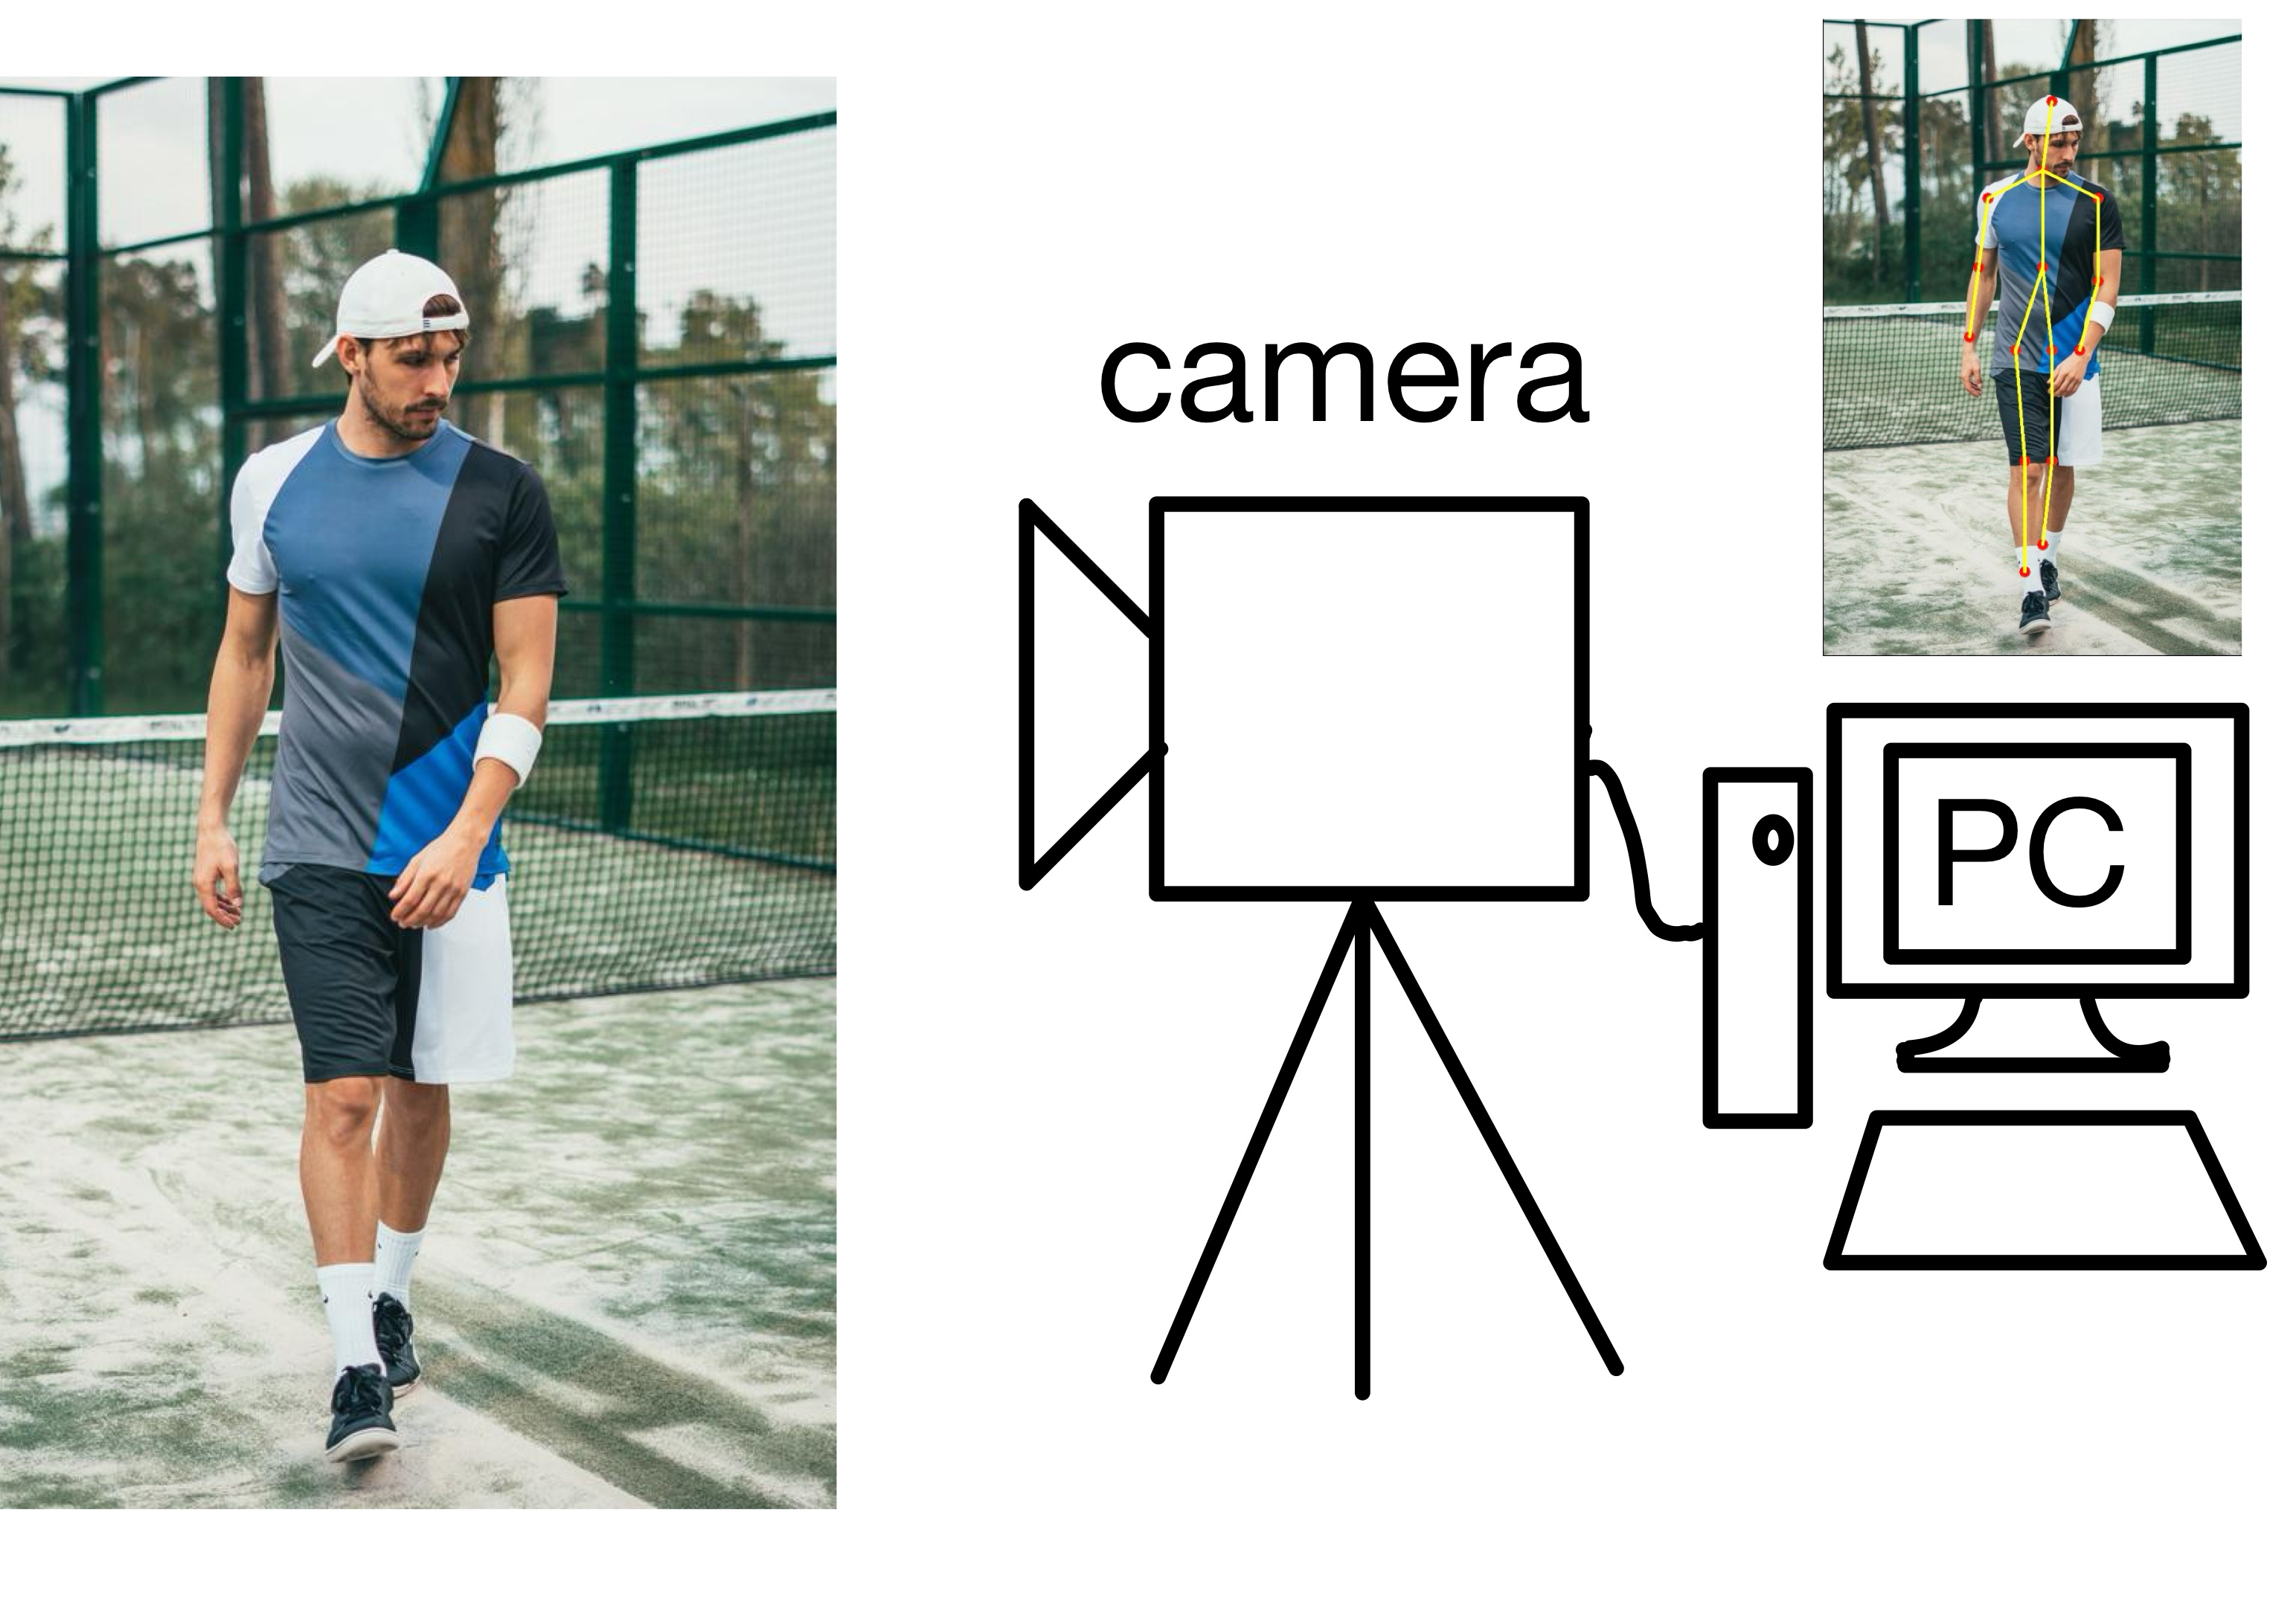
\includegraphics[width=6cm]{img/image_3D.jpg}
  \caption{画像処理による骨格推定の様子}
  \label{image_3D}
\end{figure}

画像処理による方法として2つの方法を実装する.

1つ目はカラー画像を入力としてGoogleが提供するオープンソースの機械学習ライブラリMediaPipe Poseを用いることで図\ref{RGB}に示す33個の関節の三次元骨格情報を取得する方法である.

2つ目はカラー画像とデプス情報を入力として3DiVi Incが提供するライブラリNuitrackを用いることで図\ref{RGBD}に示す19個の関節の三次元骨格情報を取得する方法である.
% \subsection{RGBカメラ一台を用いた三次元骨格推定}\label{RGB_sec}
% 画像入力機器としてRGBDカメラであるRealSense D415を使用し,カラー画像を入力として図\ref{RGB}に示す33個の関節が取得できる,Googleが提供するオープンソースの機械学習ライブラリMediaPipe Poseで三次元計測を行う.

% \subsection{RGBDカメラで行う三次元骨格推定}\label{RGBD_sec}
% 画像入力機器としてRGBDカメラであるRealSense D415を使用し,カラー画像と深度情報を入力として図\ref{RGBD}に示す19個の関節が取得できる,3DiVi Incが提供するNuitrackで三次元計測を行う.
\begin{figure*}[t]
  \begin{tabular}{ccc}
    \begin{minipage}[]{0.3\hsize}
      \centering
      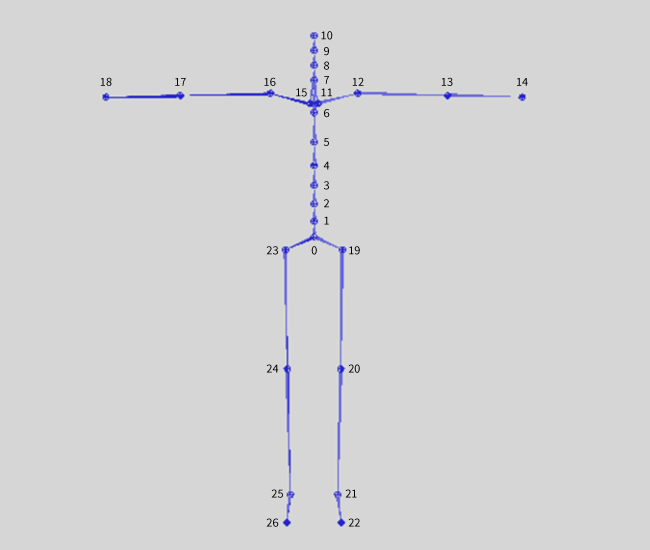
\includegraphics[height=45mm]{img/TechSpec_02.png}
      \subcaption{mocopiで取得できる関節位置}
      \label{mocopi}
    \end{minipage}
    \hspace{0.03\columnwidth} % ここで隙間作成
    \begin{minipage}[]{0.3\hsize}
      \centering
      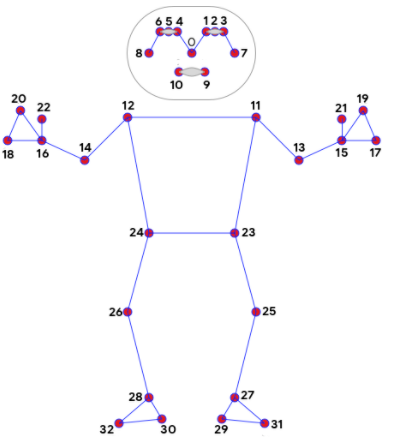
\includegraphics[height=45mm]{img/media.png}
      \subcaption{MediaPipe Poseで取得できる関節位置}
      \label{RGB}
    \end{minipage}
    \hspace{0.03\columnwidth} % ここで隙間作成
    \begin{minipage}[]{0.3\hsize}
      \centering
      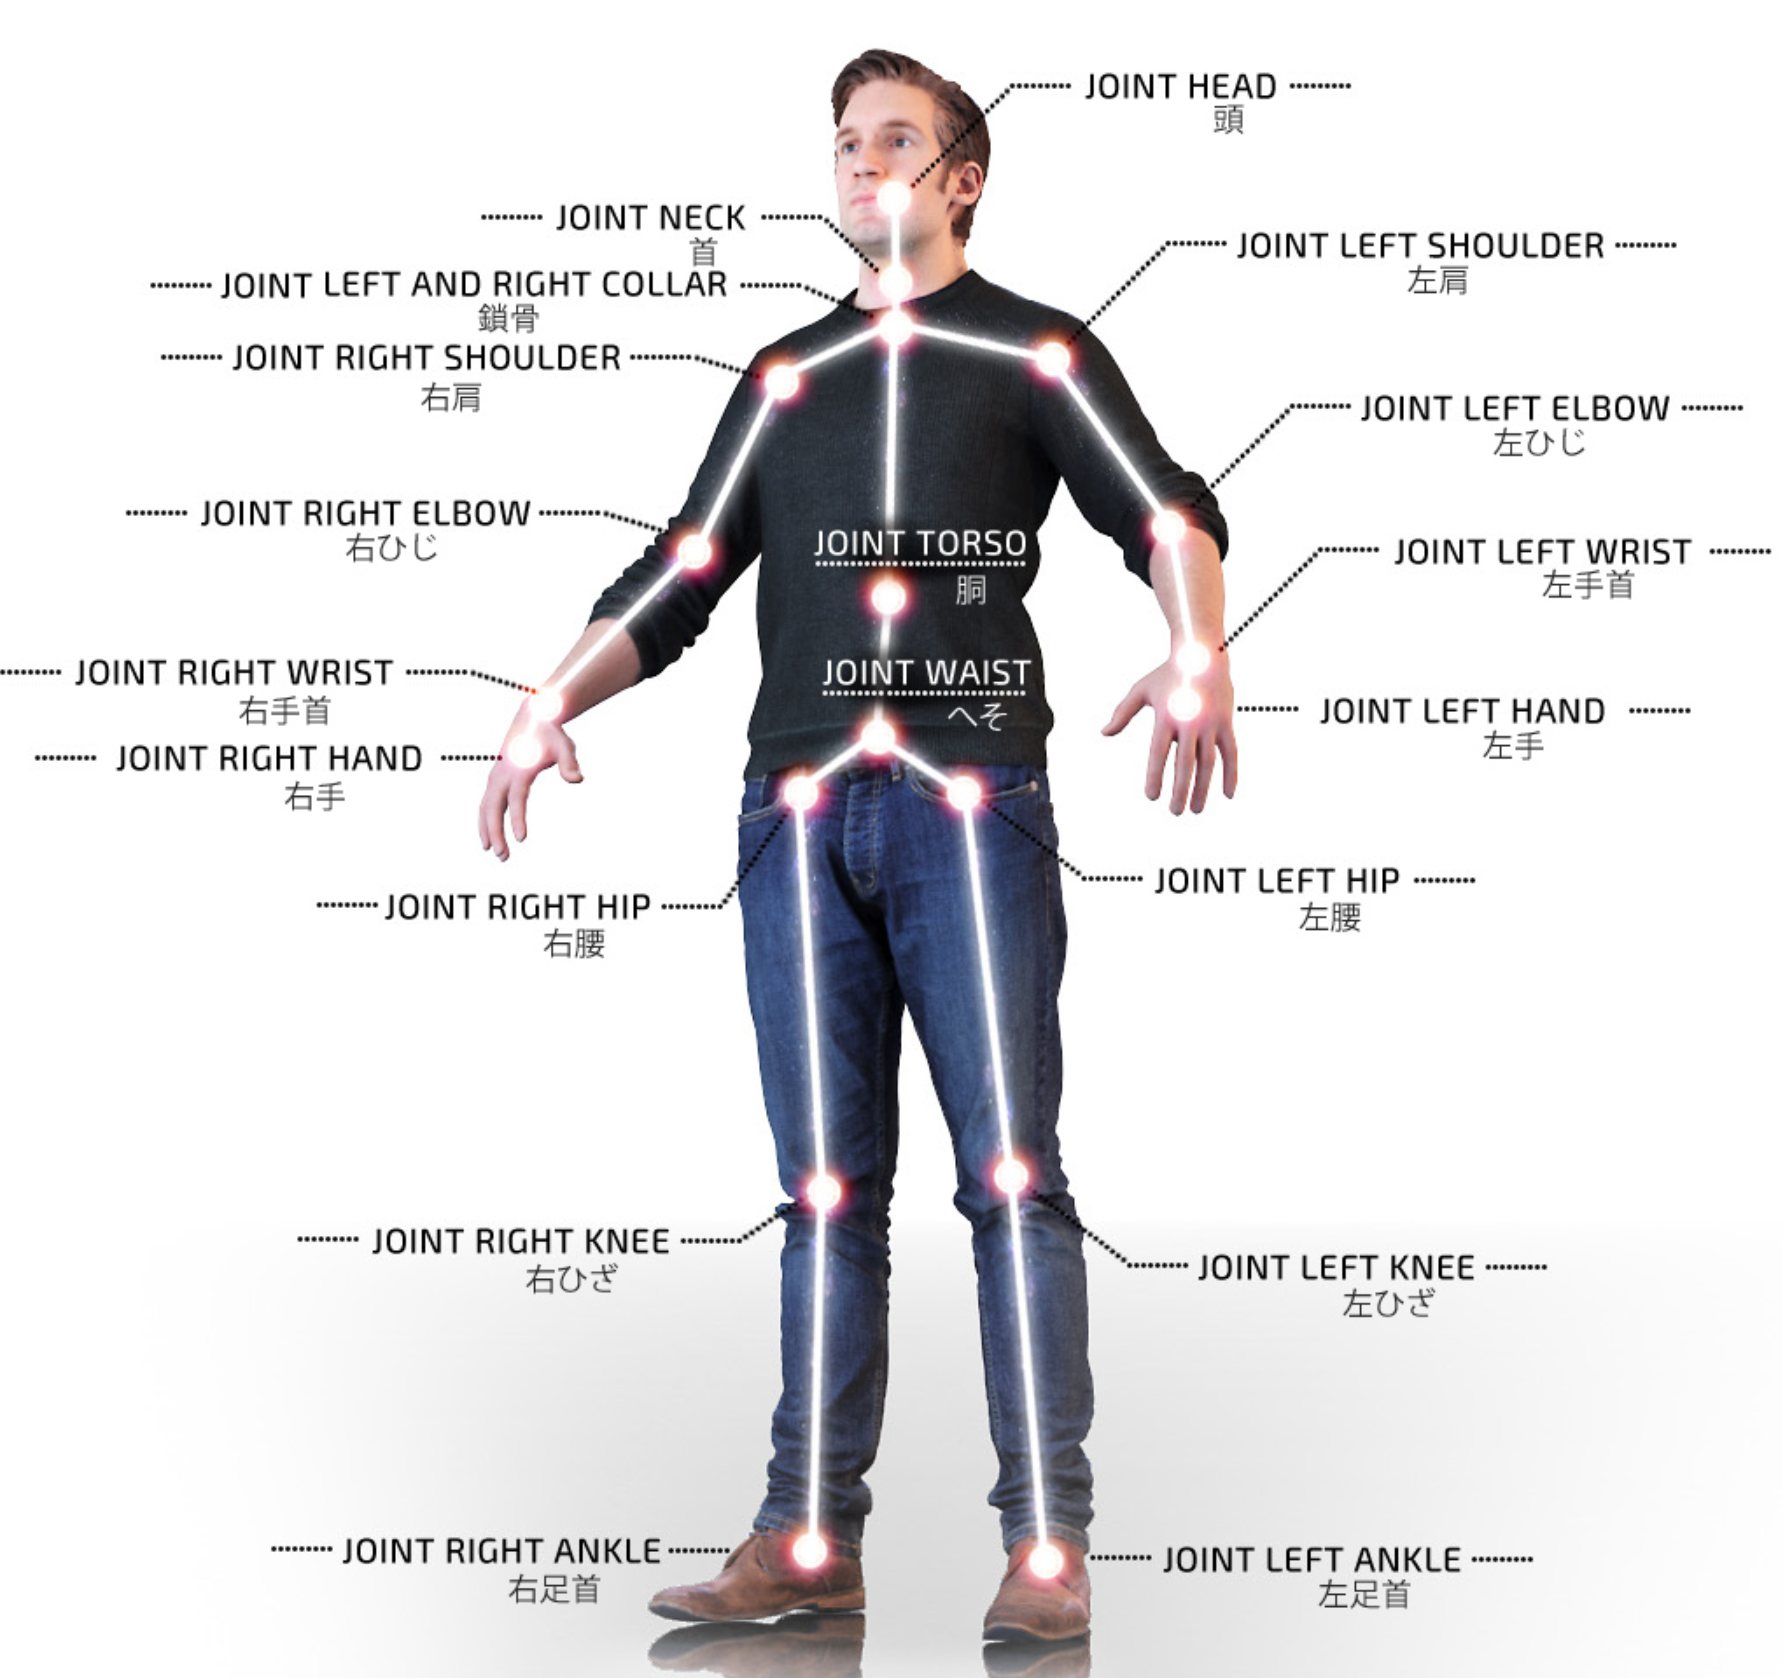
\includegraphics[height=45mm]{img/nuitrack.png}
      \subcaption{Nuitrackで取得できる関節位置}
      \label{RGBD}
    \end{minipage}
  \end{tabular}
  \caption{取得できる骨格}
  \label{sokutei}
\end{figure*}

\subsection{キャリブレーション}\label{kyari}
推定方法によって骨格座標のスケールや基準となる座標系が違うので定量的に比較評価するためには座標系を統一する必要がある.
そこで計測開始時に,両腕を水平に上げるポーズを取ることにする.水平に上げた両手首の距離を元にスケールを合わせる.
また,へその位置を原点として,頭に向かう方向をy軸,右手から左手に向かう方向をx軸,これらに軸の直行する方向をz軸と定める.

動作の比較を行うには同期を取る必要があるがmocopiは同期計測ができない.
そこで座標系を合わせるポーズの後で両手を伸ばしたまま胸の前で合わせるポーズをする.
手が合わさっている時,両手首が最接近するので,各骨格情報の両手首の座標が最も近づいたフレームを時刻の基準と定める.
% 計測方法により,座標系やスケール,時間遅れが異なるので同期が必要である.
% 座標系やスケール,処理により発生した時間遅れを統一するためのキャリブレーションを行う必要がある.
% キャリブレーションの方法として計測前に両腕を水平に広げ,その後腕を伸ばしたまま両手を胸の前で合わせるポーズを取る.

% 1つ目の両腕を水平に上げるポーズを元に座標系とスケールのキャリブレーションを行う.
% 水平に上げた両手首の距離を元にスケールを合わせる.
% また,へその位置を原点として,頭に向かう方向をy軸,右手から左手に向かう方向をx軸,これらの軸と直交する方向をz軸として座標系を定める.

% 2つ目の両手を伸ばしたまま胸の前で合わせるポーズでは,両手首が最接近していることを利用する.各骨格情報の両手首の座標が最も近づいたフレームを合わせることで時間遅れを修正する.
\section{研究結果}
\subsection{実験方法}
% 全身運動をしている人物一人に対して計測を行い,mocopiのセンサの位置に当たる両手,両足,頭,腰の計6ヶ所に関して,画像処理を用いた三次元骨格推定で得られた座標との誤差を比較することで精度を評価する.
全身運動をしている一名の被験者(男子学生)が(\ref{kyari})に示す骨格情報のキャリブレーションに必要なポーズを行い,正しくキャリブレーションできているか骨格データを評価する.
手を広げた状態から手を合わせるポーズになるまでは170フレームで行われている.
手を広げたポーズを取ったとき,へそを原点,体の中心から右手首までの距離を1としたx-z平面で表す.
\subsection{解析結果}
% RGB画像により取得した骨格データと慣性式モーションキャプチャにより取得した骨格データのキャリブレーション時の右手の座標の結果をxz平面に並べた結果を図\ref{fig:1_media},\ref{fig:1_mocopi}に示す.
mocopiにより取得した右手首の骨格座標情報を図\ref{fig:1_mocopi},mediapipeにより取得した右手首の骨格座標情報を図\ref{fig:1_media}に示す.

\begin{figure}[h]
  \centering
  \begin{minipage}{6cm}
    \centering
    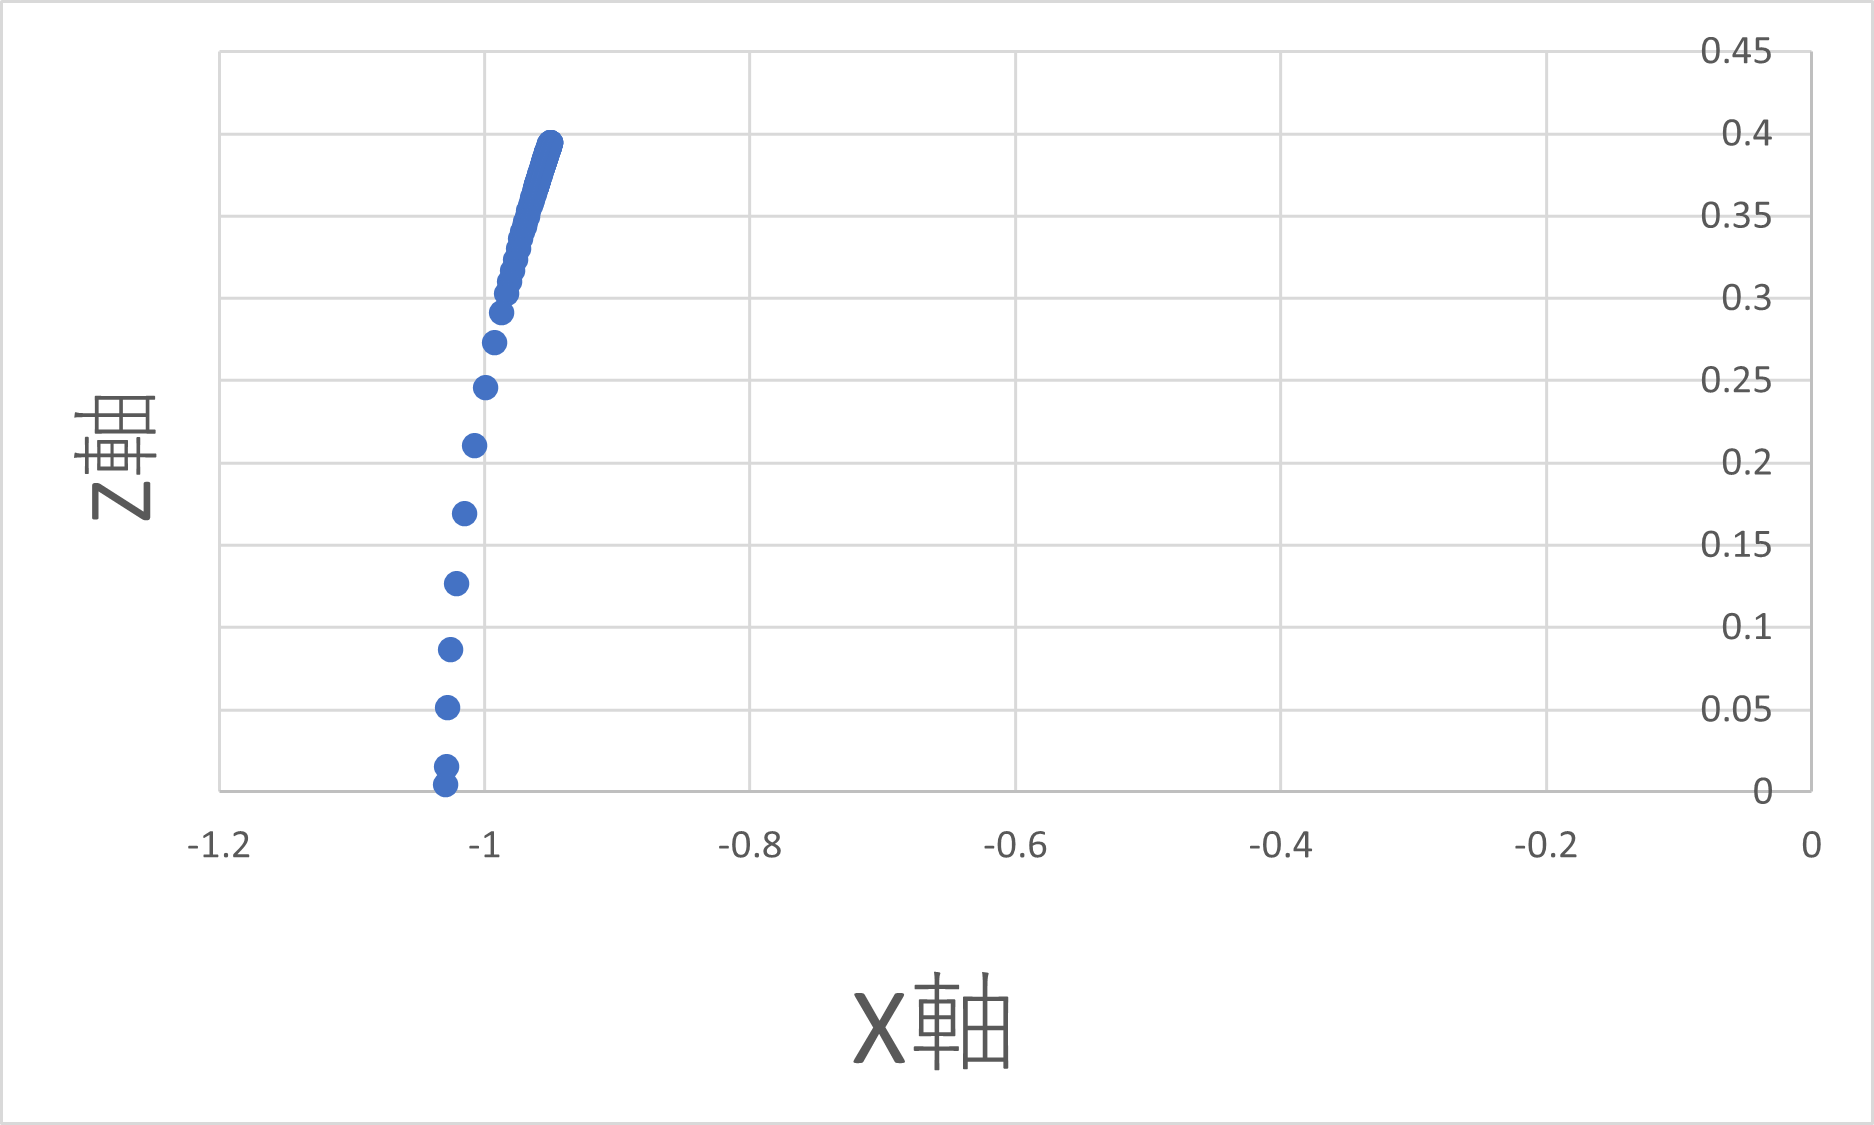
\includegraphics[width=6cm]{img/1_mocopi.png}
    \caption{mocopiで得た右手首の位置情報}
    \label{fig:1_mocopi}
  \end{minipage}\\
  \begin{minipage}{6cm}
    \centering
    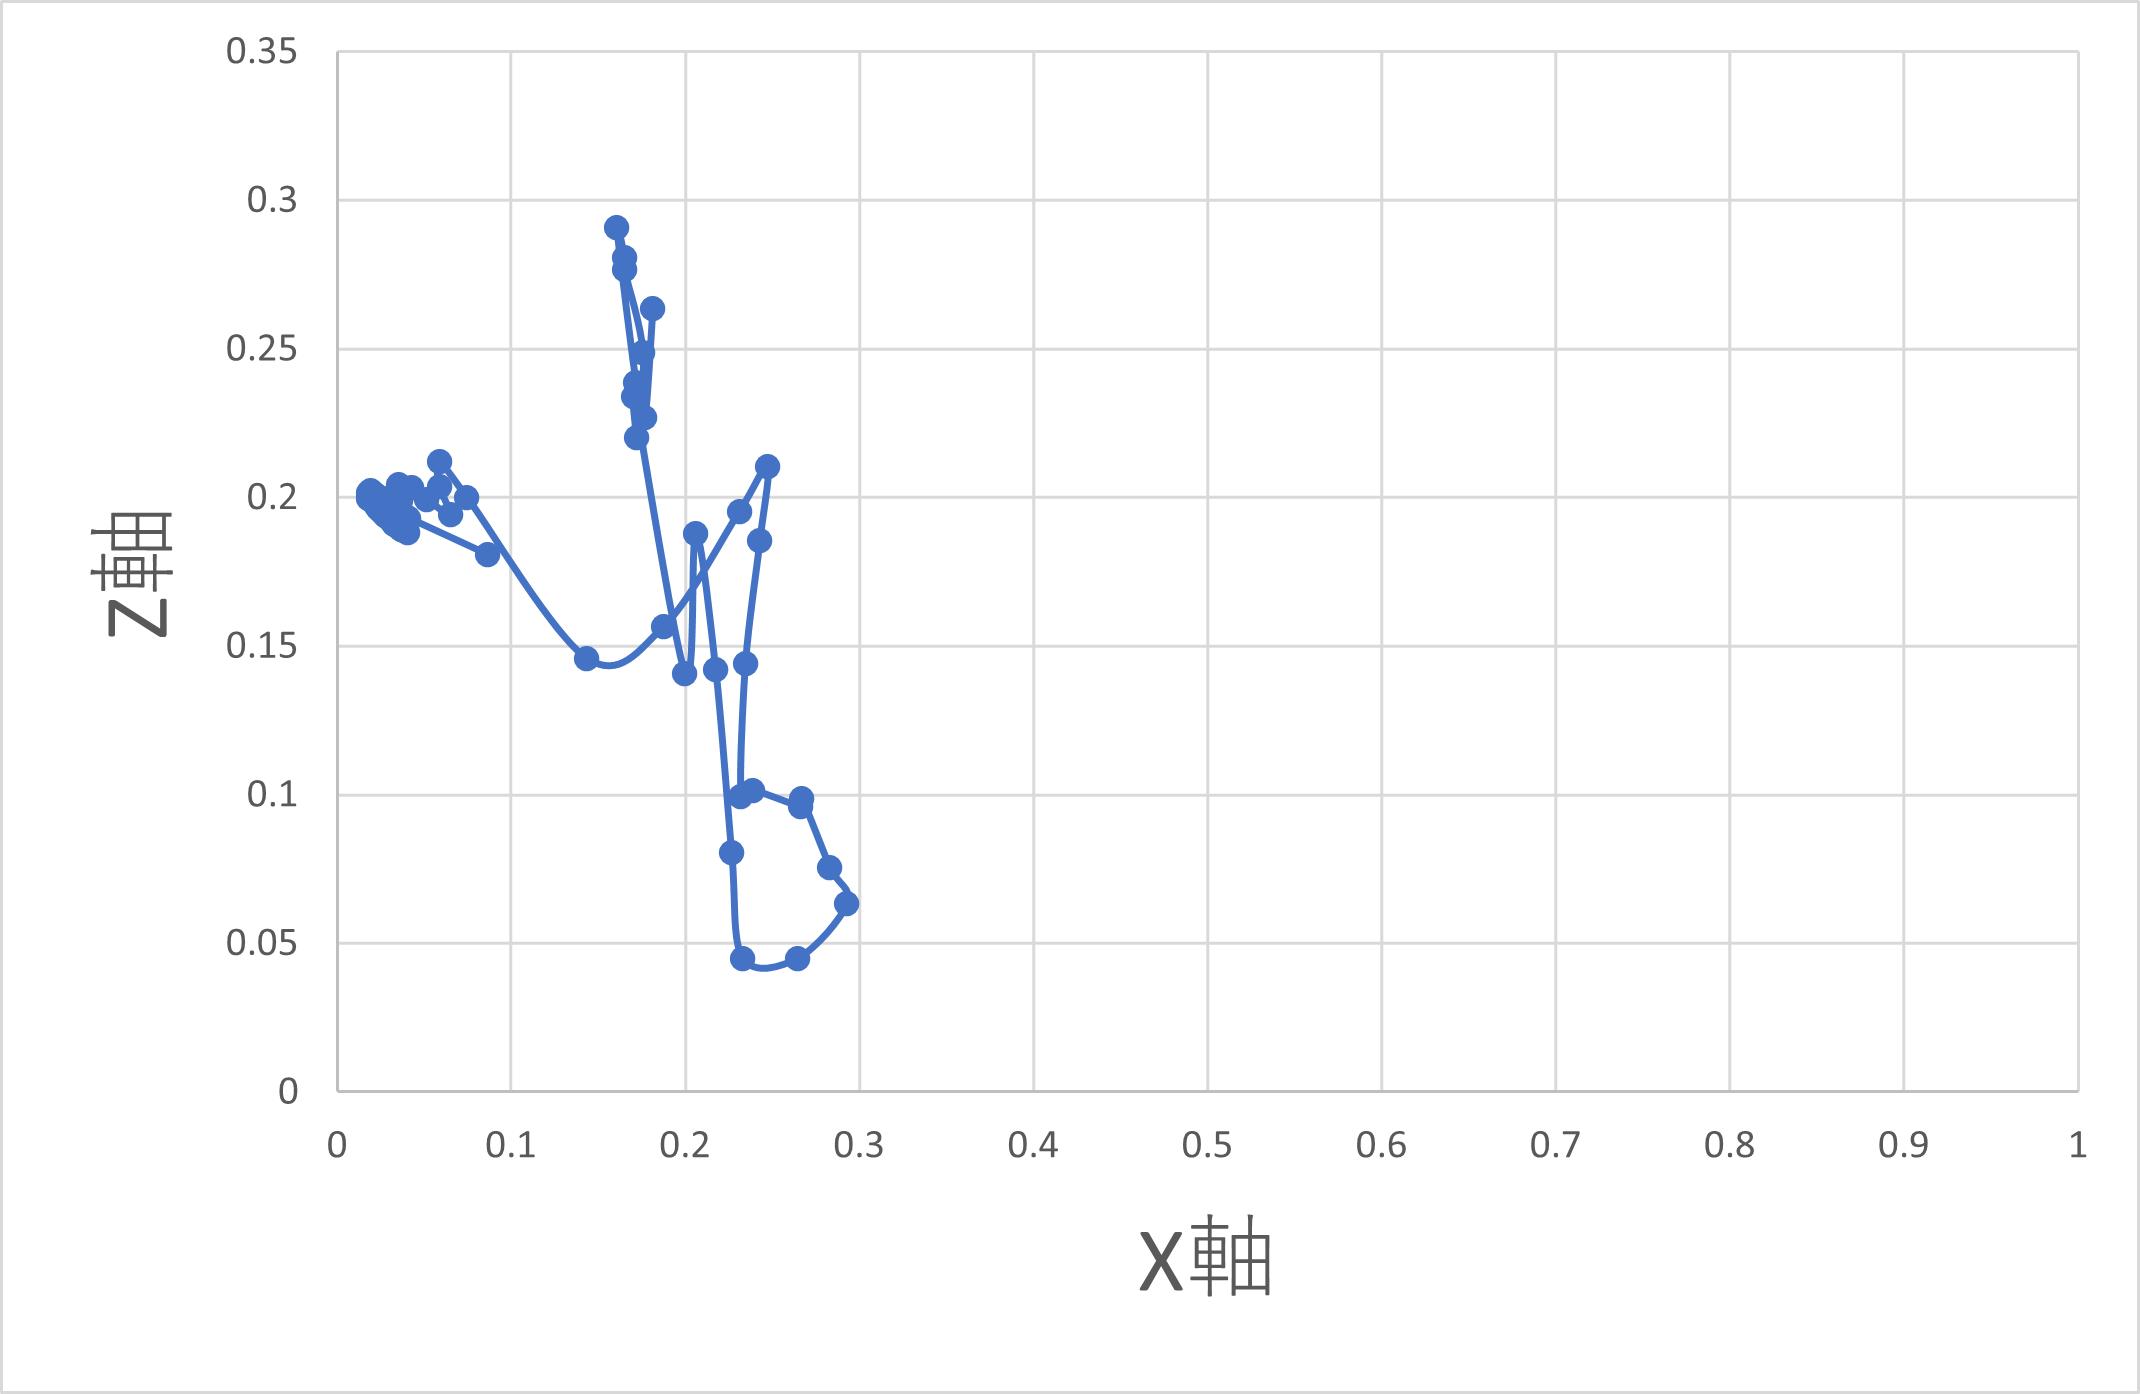
\includegraphics[width=6cm]{img/1_media.png}
    \caption{mediapipeで得た右手首の位置情報}
    \label{fig:1_media}
  \end{minipage}
\end{figure}

今回行った運動では,へそより前に右手首が存在しているため,z軸方向の値が負になることはありえない.
また,へその前まで腕を持ってきているので,正しく計測できていれば原点を中心とした半径位置の円に似た軌道を描くはずである.
mocopiは奥行きに縮んでいることがわかる.ジェスチャーのような大まかな体の動きは分かるが,センサ位置の絶対的な座標は出していないことが分かった.
RGB画像による方法では,奥行きに歪んでいることに加え,z軸方向の値が負になっている場面があるため,z軸方向の計測値に大きな誤差があることが分かる.
どちらも課題が残る結果になった.
% このような人体の恒常性があるのか怪しい結果になってしまった.
% このような結果になった原因として,キャリブレーションに用いた計測ポーズがキャリブレーションの方法と相性が悪い可能性や誤差を含みやすいものだった可能性が挙げられる.
\section{まとめ}
本研究では,キャリブレーションの方法として2つのポーズを続けて行い,3種類の手法を定量的に比較するためのキャリブレーションを試みた.
RGBカメラによる方法では機械学習を用いて奥行き情報を取得できる方法を用いたが,慣性式モーションキャプチャデバイスで取得した骨格データより精度が下がることが確認できた.

RGBDによる方法では現在問題の修正中であるがRGBDによる方法を用いることで.デプス情報を元に正しく測定できるのではないかと考えられる.
\begin{thebibliography}{99}
  \small{
    \bibitem{turugi}{
      剱 一輝,``柔道競技の3Dアーカイブ化'',令和4年度長岡高専専攻科論文,2023.
    }
    \bibitem{mediapipe}{
      Google,``mediapipe'',\\
      \url{https://developers.google.com/mediapipe}
    }
    \bibitem{depth}{
      北川リサ,伊藤貴之,``競技かるたにおける払いの動作の三次元ボーン表示による可視化'',情報処理学会第85回全国大会,
      2023,1,139 -- 140,2023.
    }
    % \bibitem{open}{
    %   サンプル画像``single.jpeg'',\url{https://github.com/spmallick/learnopencv/blob/master/OpenPose/single.jpeg}
    % }
  }
\end{thebibliography}
\rightline{URLは2023年1月25日にアクセス}
\end{document}